\documentclass[../main.tex]{subfiles}
\begin{document}
\subsection{Comparing exchange versus no exchange}
One of the objectives is to find out whether exchanging parcels between agents is benifical with respect to the objective function.
In figure \ref{fig:exch} the results of running all data sets, ceteris paribus, with and without exchanges enabled are displayed.
There is no clear difference which choice is better only 8 of the 15 datasets yields better results with the exchanges enabled.
Note however that this could be due to the way we implemented the exchange. 
The implemenation is quite naive and tries to exchange very often. 
An improvement could be looking at how much distance would be covered between the parcels in both agents and only exchange if the new clustering would improve this number.
The averages in table \ref{tab:avgstrat} also ar
\begin{figure}
	\centering
	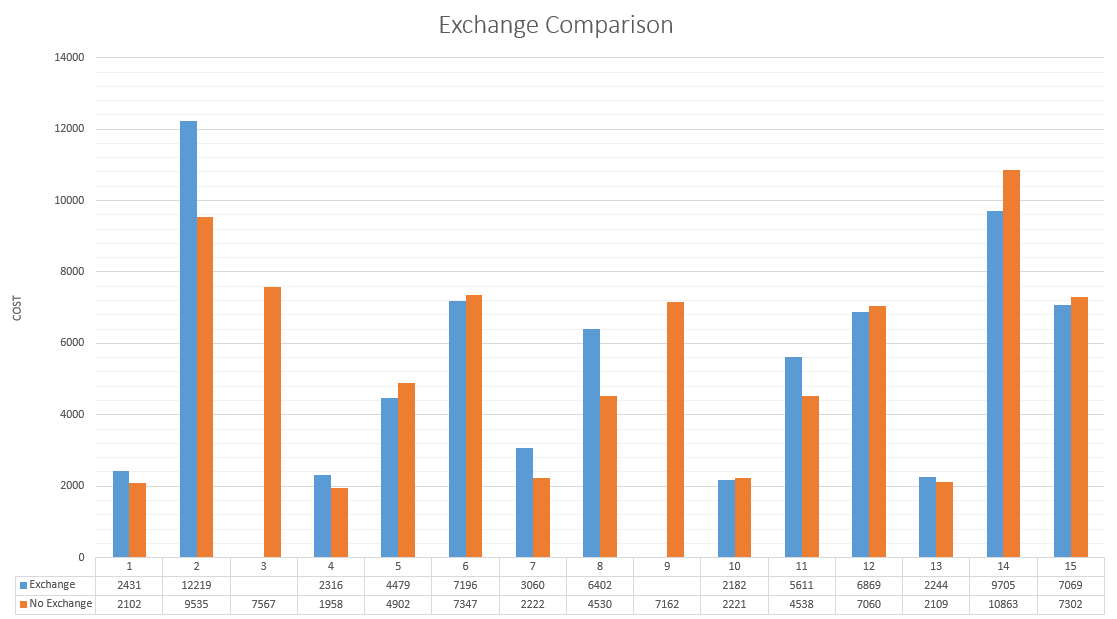
\includegraphics[width=\textwidth]{exchangecomp.png}
	\caption{Visual representation of comparing experiments with and without exchanges between agents.}
	\label{fig:exch}
\end{figure}

\begin{table}
\begin{tabular}{lcc}
	& Without Exchange & With Exchange \\ 
	EarliestDeadlineStrategy & 5366 & 5666.8 \\ 
	NearestDeliveryStrategy & 5427.867 & 5558,357 \\ 
	NearestOnTimeDeliveryStrategy & 5323.929 & 5189.615 \\ 
\end{tabular}

\caption{Table with averages of the different delivery strategies across the all data sets.}
\label{tab:avgstrat}
\end{table}

\begin{figure}
	\centering
	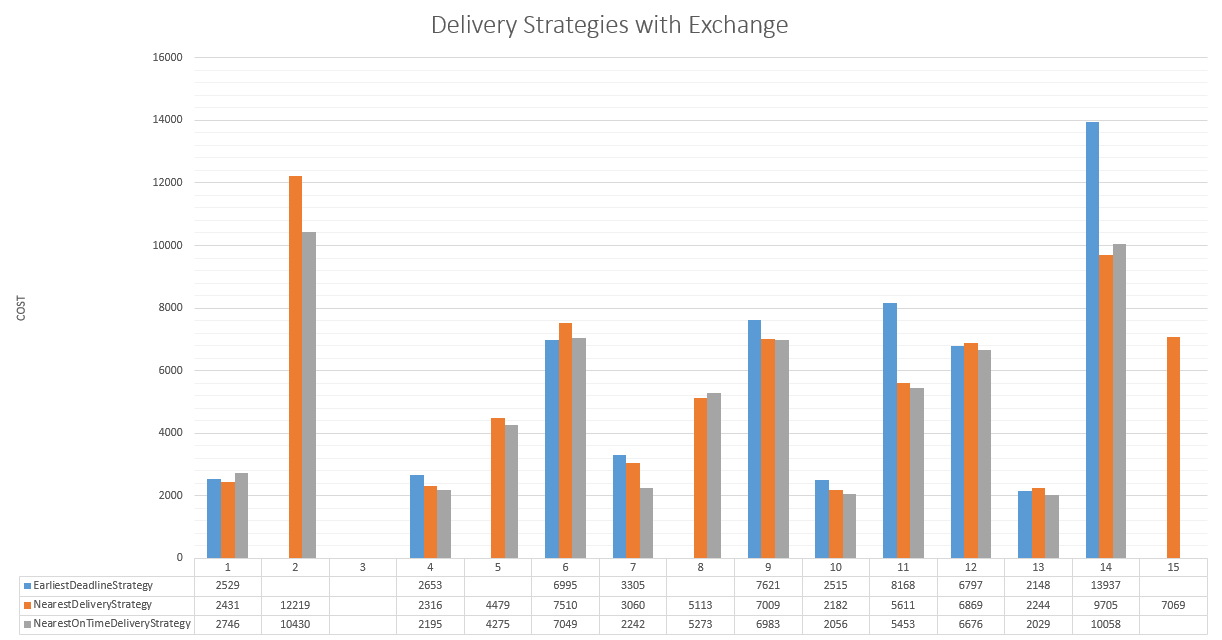
\includegraphics[width=\textwidth]{exchangestrategy.png}
	\caption{The averages taken over all dataset per beacon radius with the following levels:}
	\label{fig:strat_ex}
\end{figure}

\begin{figure}
	\centering
	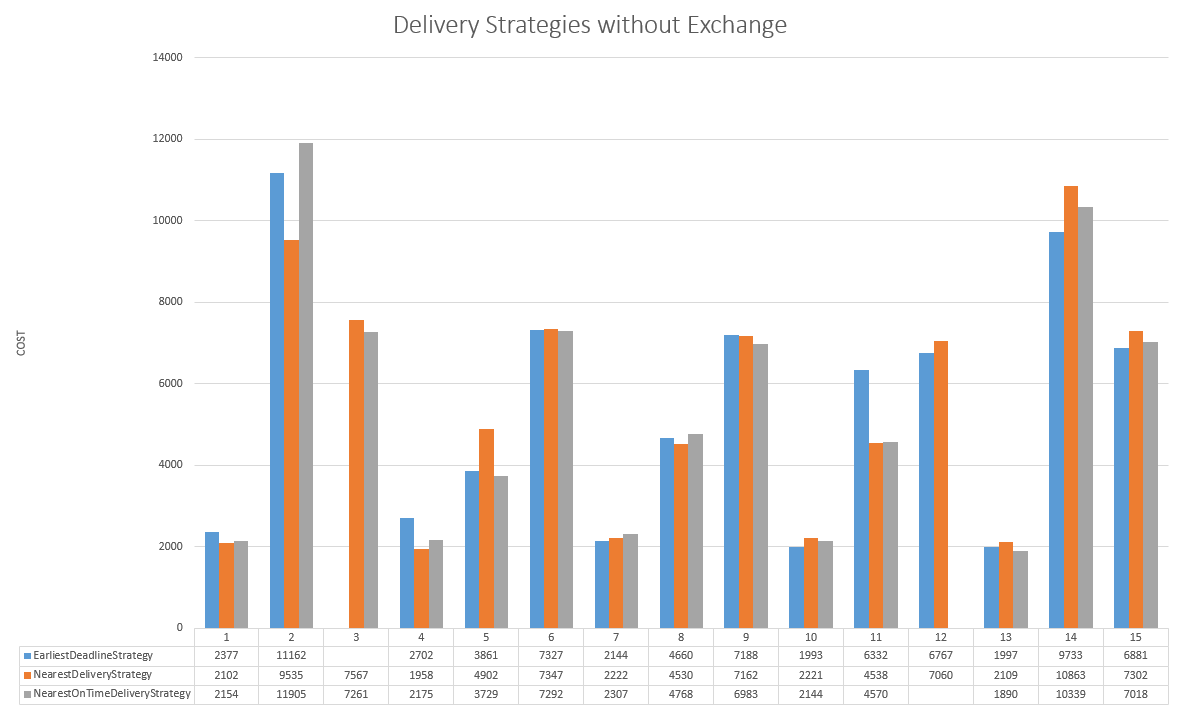
\includegraphics[width=\textwidth]{noexchangestrategy.png}
	\caption{The averages taken over all dataset per beacon radius with the following levels:}
	\label{fig:strat_noex}
\end{figure}

\begin{figure}
	\centering
	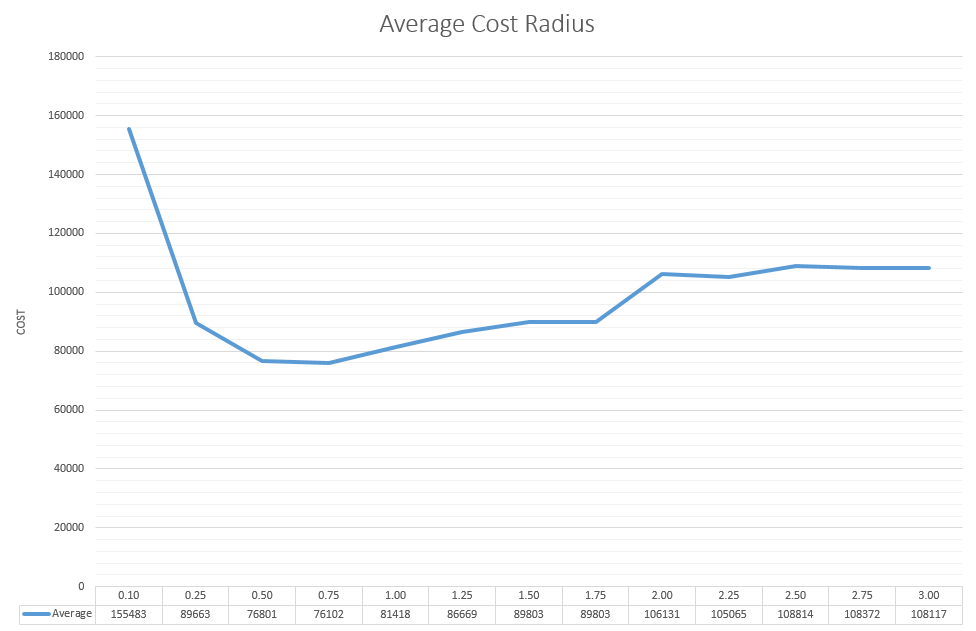
\includegraphics[width=\textwidth]{radiusaveragecost.png}
	\caption{The averages taken over all dataset per beacon radius with the following levels:}
	\label{fig:rad}
\end{figure}
\end{document}
